% Options for packages loaded elsewhere
\PassOptionsToPackage{unicode}{hyperref}
\PassOptionsToPackage{hyphens}{url}
%
\documentclass[
]{article}
\usepackage{amsmath,amssymb}
\usepackage{lmodern}
\usepackage{iftex}
\ifPDFTeX
  \usepackage[T1]{fontenc}
  \usepackage[utf8]{inputenc}
  \usepackage{textcomp} % provide euro and other symbols
\else % if luatex or xetex
  \usepackage{unicode-math}
  \defaultfontfeatures{Scale=MatchLowercase}
  \defaultfontfeatures[\rmfamily]{Ligatures=TeX,Scale=1}
\fi
% Use upquote if available, for straight quotes in verbatim environments
\IfFileExists{upquote.sty}{\usepackage{upquote}}{}
\IfFileExists{microtype.sty}{% use microtype if available
  \usepackage[]{microtype}
  \UseMicrotypeSet[protrusion]{basicmath} % disable protrusion for tt fonts
}{}
\makeatletter
\@ifundefined{KOMAClassName}{% if non-KOMA class
  \IfFileExists{parskip.sty}{%
    \usepackage{parskip}
  }{% else
    \setlength{\parindent}{0pt}
    \setlength{\parskip}{6pt plus 2pt minus 1pt}}
}{% if KOMA class
  \KOMAoptions{parskip=half}}
\makeatother
\usepackage{xcolor}
\usepackage[margin=1in]{geometry}
\usepackage{color}
\usepackage{fancyvrb}
\newcommand{\VerbBar}{|}
\newcommand{\VERB}{\Verb[commandchars=\\\{\}]}
\DefineVerbatimEnvironment{Highlighting}{Verbatim}{commandchars=\\\{\}}
% Add ',fontsize=\small' for more characters per line
\usepackage{framed}
\definecolor{shadecolor}{RGB}{248,248,248}
\newenvironment{Shaded}{\begin{snugshade}}{\end{snugshade}}
\newcommand{\AlertTok}[1]{\textcolor[rgb]{0.94,0.16,0.16}{#1}}
\newcommand{\AnnotationTok}[1]{\textcolor[rgb]{0.56,0.35,0.01}{\textbf{\textit{#1}}}}
\newcommand{\AttributeTok}[1]{\textcolor[rgb]{0.77,0.63,0.00}{#1}}
\newcommand{\BaseNTok}[1]{\textcolor[rgb]{0.00,0.00,0.81}{#1}}
\newcommand{\BuiltInTok}[1]{#1}
\newcommand{\CharTok}[1]{\textcolor[rgb]{0.31,0.60,0.02}{#1}}
\newcommand{\CommentTok}[1]{\textcolor[rgb]{0.56,0.35,0.01}{\textit{#1}}}
\newcommand{\CommentVarTok}[1]{\textcolor[rgb]{0.56,0.35,0.01}{\textbf{\textit{#1}}}}
\newcommand{\ConstantTok}[1]{\textcolor[rgb]{0.00,0.00,0.00}{#1}}
\newcommand{\ControlFlowTok}[1]{\textcolor[rgb]{0.13,0.29,0.53}{\textbf{#1}}}
\newcommand{\DataTypeTok}[1]{\textcolor[rgb]{0.13,0.29,0.53}{#1}}
\newcommand{\DecValTok}[1]{\textcolor[rgb]{0.00,0.00,0.81}{#1}}
\newcommand{\DocumentationTok}[1]{\textcolor[rgb]{0.56,0.35,0.01}{\textbf{\textit{#1}}}}
\newcommand{\ErrorTok}[1]{\textcolor[rgb]{0.64,0.00,0.00}{\textbf{#1}}}
\newcommand{\ExtensionTok}[1]{#1}
\newcommand{\FloatTok}[1]{\textcolor[rgb]{0.00,0.00,0.81}{#1}}
\newcommand{\FunctionTok}[1]{\textcolor[rgb]{0.00,0.00,0.00}{#1}}
\newcommand{\ImportTok}[1]{#1}
\newcommand{\InformationTok}[1]{\textcolor[rgb]{0.56,0.35,0.01}{\textbf{\textit{#1}}}}
\newcommand{\KeywordTok}[1]{\textcolor[rgb]{0.13,0.29,0.53}{\textbf{#1}}}
\newcommand{\NormalTok}[1]{#1}
\newcommand{\OperatorTok}[1]{\textcolor[rgb]{0.81,0.36,0.00}{\textbf{#1}}}
\newcommand{\OtherTok}[1]{\textcolor[rgb]{0.56,0.35,0.01}{#1}}
\newcommand{\PreprocessorTok}[1]{\textcolor[rgb]{0.56,0.35,0.01}{\textit{#1}}}
\newcommand{\RegionMarkerTok}[1]{#1}
\newcommand{\SpecialCharTok}[1]{\textcolor[rgb]{0.00,0.00,0.00}{#1}}
\newcommand{\SpecialStringTok}[1]{\textcolor[rgb]{0.31,0.60,0.02}{#1}}
\newcommand{\StringTok}[1]{\textcolor[rgb]{0.31,0.60,0.02}{#1}}
\newcommand{\VariableTok}[1]{\textcolor[rgb]{0.00,0.00,0.00}{#1}}
\newcommand{\VerbatimStringTok}[1]{\textcolor[rgb]{0.31,0.60,0.02}{#1}}
\newcommand{\WarningTok}[1]{\textcolor[rgb]{0.56,0.35,0.01}{\textbf{\textit{#1}}}}
\usepackage{longtable,booktabs,array}
\usepackage{calc} % for calculating minipage widths
% Correct order of tables after \paragraph or \subparagraph
\usepackage{etoolbox}
\makeatletter
\patchcmd\longtable{\par}{\if@noskipsec\mbox{}\fi\par}{}{}
\makeatother
% Allow footnotes in longtable head/foot
\IfFileExists{footnotehyper.sty}{\usepackage{footnotehyper}}{\usepackage{footnote}}
\makesavenoteenv{longtable}
\usepackage{graphicx}
\makeatletter
\def\maxwidth{\ifdim\Gin@nat@width>\linewidth\linewidth\else\Gin@nat@width\fi}
\def\maxheight{\ifdim\Gin@nat@height>\textheight\textheight\else\Gin@nat@height\fi}
\makeatother
% Scale images if necessary, so that they will not overflow the page
% margins by default, and it is still possible to overwrite the defaults
% using explicit options in \includegraphics[width, height, ...]{}
\setkeys{Gin}{width=\maxwidth,height=\maxheight,keepaspectratio}
% Set default figure placement to htbp
\makeatletter
\def\fps@figure{htbp}
\makeatother
\setlength{\emergencystretch}{3em} % prevent overfull lines
\providecommand{\tightlist}{%
  \setlength{\itemsep}{0pt}\setlength{\parskip}{0pt}}
\setcounter{secnumdepth}{-\maxdimen} % remove section numbering
\ifLuaTeX
  \usepackage{selnolig}  % disable illegal ligatures
\fi
\IfFileExists{bookmark.sty}{\usepackage{bookmark}}{\usepackage{hyperref}}
\IfFileExists{xurl.sty}{\usepackage{xurl}}{} % add URL line breaks if available
\urlstyle{same} % disable monospaced font for URLs
\hypersetup{
  pdftitle={New Data Analysis},
  pdfauthor={Jiayi Yang},
  hidelinks,
  pdfcreator={LaTeX via pandoc}}

\title{New Data Analysis}
\author{Jiayi Yang}
\date{2022-11-16}

\begin{document}
\maketitle

\begin{Shaded}
\begin{Highlighting}[]
\FunctionTok{library}\NormalTok{(}\StringTok{"MatchIt"}\NormalTok{)}
\FunctionTok{library}\NormalTok{(survival)}
\FunctionTok{library}\NormalTok{(gtsummary)}
\end{Highlighting}
\end{Shaded}

import the new data

\begin{Shaded}
\begin{Highlighting}[]
\NormalTok{new\_data }\OtherTok{=} 
  \FunctionTok{read\_excel}\NormalTok{(}\StringTok{"./LDA.xlsx"}\NormalTok{, }\AttributeTok{sheet =} \DecValTok{1}\NormalTok{, }\AttributeTok{range =} \FunctionTok{cell\_cols}\NormalTok{(}\StringTok{"A:K"}\NormalTok{)) }\SpecialCharTok{\%\textgreater{}\%} 
  \FunctionTok{filter}\NormalTok{(flo\_meas\_name }\SpecialCharTok{\%in\%} \FunctionTok{c}\NormalTok{(  }\StringTok{\textquotesingle{}G IP NYC LDA MIDLINE DOUBLE LUMEN\textquotesingle{}}\NormalTok{,}
                                \StringTok{\textquotesingle{}G IP NYC LDA MIDLINE SINGLE LUMEN\textquotesingle{}}\NormalTok{,}
                                \StringTok{\textquotesingle{}G LDA PULMONARY ARTERY CATHETER/SWAN GANZ\textquotesingle{}}\NormalTok{,}
                                \StringTok{\textquotesingle{}LDA CVC QUADRUPLE LUMEN\textquotesingle{}}\NormalTok{,}
                                \StringTok{\textquotesingle{}LDA CVC SINGLE LUMEN\textquotesingle{}}\NormalTok{,}
                                \StringTok{\textquotesingle{}LDA CVC TRIPLE LUMEN\textquotesingle{}}\NormalTok{,}
                                \StringTok{\textquotesingle{}LDA DUAL LUMEN PORT\textquotesingle{}}\NormalTok{,}
                                \StringTok{\textquotesingle{}LDA EXTERNAL URINARY CATHETER\textquotesingle{}}\NormalTok{,}
                                \StringTok{\textquotesingle{}LDA PICC SINGLE LUMEN\textquotesingle{}}\NormalTok{,}
                                \StringTok{\textquotesingle{}LDA PICC TRIPLE LUMEN\textquotesingle{}}\NormalTok{,}
                                \StringTok{\textquotesingle{}LDA PUMP DEVICE\textquotesingle{}}\NormalTok{,}
                                \StringTok{\textquotesingle{}NYC LDA PRESSURE INJURY\textquotesingle{}}\NormalTok{,}
                                \StringTok{\textquotesingle{}RETIRED {-} NYC ADT TC PICC DOUBLE LUMEN\textquotesingle{}}\NormalTok{)}
\NormalTok{         ) }\SpecialCharTok{\%\textgreater{}\%} 
  \FunctionTok{mutate}\NormalTok{(}
    \AttributeTok{placement\_date =} \FunctionTok{as.Date}\NormalTok{(PLACEMENT\_INSTANT, }\StringTok{"\%y/\%m/\%d"}\NormalTok{),}
    \AttributeTok{removal\_date =} \FunctionTok{as.Date}\NormalTok{(REMOVAL\_INSTANT, }\StringTok{"\%y/\%m/\%d"}\NormalTok{),}
    \AttributeTok{duration =}\NormalTok{ removal\_date }\SpecialCharTok{{-}}\NormalTok{ placement\_date}
\NormalTok{  ) }\SpecialCharTok{\%\textgreater{}\%} 
  \FunctionTok{filter}\NormalTok{(removal\_date }\SpecialCharTok{!=} \StringTok{\textquotesingle{}2157{-}11{-}19\textquotesingle{}}\NormalTok{)}
\end{Highlighting}
\end{Shaded}

\begin{verbatim}
## Warning in as.POSIXlt.POSIXct(x, tz = tz): unknown timezone '%y/%m/%d'

## Warning in as.POSIXlt.POSIXct(x, tz = tz): unknown timezone '%y/%m/%d'
\end{verbatim}

\begin{Shaded}
\begin{Highlighting}[]
\NormalTok{new\_data}
\end{Highlighting}
\end{Shaded}

\begin{verbatim}
## # A tibble: 6,754 x 14
##          EMPI BIRTH_DATE          sex_c PAT_ENC_CSN_ID hosp_admsn_time    
##         <dbl> <dttm>              <dbl>          <dbl> <dttm>             
##  1 1000039263 1937-04-28 00:00:00     2      115794137 2020-02-05 01:08:00
##  2 1000087431 1945-05-18 00:00:00     1      150005039 2021-07-02 15:08:00
##  3 1000087431 1945-05-18 00:00:00     1      150005039 2021-07-02 15:08:00
##  4 1000092404 1942-03-24 00:00:00     1      190464289 2022-05-07 10:23:00
##  5 1000092404 1942-03-24 00:00:00     1      190464289 2022-05-07 10:23:00
##  6 1000172922 1950-09-19 00:00:00     1      186868549 2022-03-31 22:09:00
##  7 1000178374 1987-03-12 00:00:00     2      179436960 2022-01-10 02:25:00
##  8 1000039263 1937-04-28 00:00:00     2      115794137 2020-02-05 01:08:00
##  9 1000039263 1937-04-28 00:00:00     2      115794137 2020-02-05 01:08:00
## 10 1000087431 1945-05-18 00:00:00     1      150005039 2021-07-02 15:08:00
## # ... with 6,744 more rows, and 9 more variables: hosp_disch_time <dttm>,
## #   FLO_MEAS_ID <dbl>, PLACEMENT_INSTANT <dttm>, REMOVAL_INSTANT <dttm>,
## #   DESCRIPTION <chr>, flo_meas_name <chr>, placement_date <date>,
## #   removal_date <date>, duration <drtn>
\end{verbatim}

\begin{Shaded}
\begin{Highlighting}[]
\NormalTok{new\_data2 }\OtherTok{=}\NormalTok{ new\_data[}\SpecialCharTok{!}\FunctionTok{duplicated}\NormalTok{(new\_data}\SpecialCharTok{$}\NormalTok{EMPI), ] }\SpecialCharTok{\%\textgreater{}\%} \FunctionTok{drop\_na}\NormalTok{()}
\NormalTok{duration\_sum }\OtherTok{\textless{}{-}} \FunctionTok{aggregate}\NormalTok{(new\_data2}\SpecialCharTok{$}\NormalTok{duration, }\AttributeTok{by =} \FunctionTok{list}\NormalTok{(new\_data2}\SpecialCharTok{$}\NormalTok{EMPI), }\AttributeTok{FUN =}\NormalTok{ sum)}
\FunctionTok{str\_remove}\NormalTok{(duration\_sum}\SpecialCharTok{$}\NormalTok{x,}\StringTok{"days"}\NormalTok{)}
\end{Highlighting}
\end{Shaded}

\begin{verbatim}
##    [1] "3"   "2"   "0"   "5"   "10"  "9"   "6"   "3"   "17"  "15"  "3"   "8"  
##   [13] "3"   "8"   "1"   "3"   "1"   "20"  "2"   "7"   "2"   "0"   "0"   "14" 
##   [25] "3"   "13"  "17"  "14"  "2"   "7"   "2"   "4"   "8"   "6"   "5"   "4"  
##   [37] "35"  "9"   "8"   "45"  "2"   "0"   "14"  "5"   "4"   "12"  "7"   "8"  
##   [49] "18"  "6"   "4"   "15"  "4"   "17"  "19"  "21"  "5"   "11"  "4"   "16" 
##   [61] "2"   "9"   "2"   "155" "0"   "3"   "4"   "1"   "1"   "5"   "1"   "5"  
##   [73] "1"   "254" "1"   "7"   "2"   "0"   "7"   "3"   "5"   "20"  "1"   "3"  
##   [85] "3"   "1"   "3"   "2"   "2"   "1"   "2"   "4"   "1"   "9"   "14"  "4"  
##   [97] "7"   "3"   "13"  "8"   "8"   "0"   "4"   "1"   "15"  "7"   "8"   "2"  
##  [109] "4"   "1"   "0"   "2"   "3"   "4"   "6"   "4"   "7"   "1"   "0"   "3"  
##  [121] "12"  "9"   "5"   "9"   "79"  "14"  "7"   "5"   "36"  "14"  "6"   "7"  
##  [133] "14"  "1"   "13"  "3"   "13"  "7"   "7"   "11"  "9"   "4"   "6"   "7"  
##  [145] "4"   "6"   "16"  "1"   "0"   "18"  "15"  "19"  "5"   "1"   "6"   "38" 
##  [157] "2"   "6"   "1"   "10"  "6"   "8"   "11"  "1"   "13"  "9"   "11"  "37" 
##  [169] "0"   "13"  "13"  "29"  "8"   "15"  "11"  "4"   "5"   "15"  "5"   "26" 
##  [181] "1"   "1"   "2"   "0"   "1"   "7"   "0"   "0"   "2"   "9"   "10"  "4"  
##  [193] "8"   "16"  "3"   "2"   "24"  "6"   "3"   "1"   "32"  "5"   "14"  "1"  
##  [205] "7"   "2"   "9"   "1"   "6"   "6"   "44"  "22"  "2"   "5"   "11"  "1"  
##  [217] "2"   "2"   "2"   "1"   "13"  "2"   "17"  "12"  "5"   "9"   "0"   "2"  
##  [229] "8"   "6"   "16"  "2"   "3"   "7"   "16"  "219" "0"   "2"   "46"  "19" 
##  [241] "8"   "1"   "21"  "2"   "32"  "62"  "5"   "3"   "6"   "13"  "16"  "1"  
##  [253] "11"  "4"   "1"   "0"   "6"   "10"  "19"  "50"  "12"  "2"   "1"   "4"  
##  [265] "12"  "19"  "10"  "30"  "12"  "30"  "0"   "1"   "2"   "1"   "2"   "1"  
##  [277] "1"   "11"  "3"   "13"  "10"  "5"   "6"   "11"  "0"   "4"   "1"   "0"  
##  [289] "45"  "8"   "15"  "12"  "6"   "6"   "6"   "0"   "1"   "11"  "6"   "0"  
##  [301] "2"   "4"   "11"  "6"   "28"  "19"  "0"   "0"   "4"   "56"  "8"   "31" 
##  [313] "13"  "2"   "38"  "3"   "19"  "0"   "14"  "13"  "10"  "13"  "35"  "1"  
##  [325] "16"  "23"  "26"  "0"   "9"   "1"   "22"  "4"   "10"  "15"  "1"   "35" 
##  [337] "2"   "4"   "7"   "7"   "4"   "0"   "10"  "6"   "1"   "12"  "9"   "16" 
##  [349] "16"  "2"   "84"  "11"  "1"   "1"   "8"   "26"  "26"  "1"   "7"   "46" 
##  [361] "3"   "0"   "10"  "12"  "17"  "2"   "2"   "7"   "1"   "1"   "10"  "6"  
##  [373] "9"   "32"  "1"   "2"   "14"  "7"   "4"   "4"   "2"   "1"   "15"  "3"  
##  [385] "1"   "13"  "1"   "2"   "13"  "20"  "2"   "10"  "0"   "6"   "1"   "1"  
##  [397] "2"   "4"   "4"   "2"   "17"  "1"   "2"   "17"  "4"   "2"   "0"   "10" 
##  [409] "2"   "9"   "4"   "7"   "11"  "1"   "3"   "2"   "5"   "3"   "7"   "0"  
##  [421] "11"  "17"  "1"   "0"   "8"   "5"   "10"  "9"   "13"  "1"   "1"   "7"  
##  [433] "1"   "23"  "2"   "12"  "1"   "0"   "28"  "11"  "1"   "12"  "4"   "3"  
##  [445] "2"   "4"   "12"  "4"   "2"   "1"   "4"   "84"  "5"   "12"  "7"   "2"  
##  [457] "32"  "10"  "12"  "0"   "62"  "19"  "8"   "71"  "0"   "2"   "2"   "8"  
##  [469] "0"   "7"   "0"   "13"  "23"  "14"  "165" "5"   "8"   "1"   "8"   "88" 
##  [481] "3"   "3"   "0"   "14"  "13"  "7"   "1"   "1"   "4"   "2"   "5"   "0"  
##  [493] "11"  "0"   "5"   "3"   "5"   "1"   "3"   "14"  "9"   "9"   "3"   "47" 
##  [505] "108" "0"   "1"   "2"   "11"  "26"  "2"   "3"   "24"  "4"   "36"  "9"  
##  [517] "3"   "3"   "2"   "11"  "3"   "3"   "3"   "9"   "10"  "41"  "40"  "5"  
##  [529] "18"  "31"  "0"   "12"  "7"   "0"   "7"   "2"   "16"  "2"   "0"   "0"  
##  [541] "0"   "89"  "2"   "20"  "26"  "9"   "8"   "2"   "3"   "6"   "2"   "5"  
##  [553] "1"   "20"  "32"  "3"   "2"   "3"   "59"  "13"  "20"  "2"   "6"   "12" 
##  [565] "32"  "3"   "3"   "0"   "1"   "6"   "3"   "82"  "1"   "2"   "30"  "1"  
##  [577] "15"  "4"   "2"   "43"  "1"   "1"   "5"   "8"   "25"  "1"   "0"   "2"  
##  [589] "1"   "0"   "2"   "8"   "19"  "1"   "10"  "10"  "28"  "3"   "0"   "10" 
##  [601] "4"   "1"   "209" "17"  "1"   "18"  "2"   "32"  "11"  "5"   "10"  "6"  
##  [613] "5"   "5"   "7"   "14"  "3"   "29"  "3"   "18"  "9"   "12"  "11"  "1"  
##  [625] "16"  "16"  "2"   "25"  "6"   "7"   "8"   "6"   "1"   "1"   "1"   "7"  
##  [637] "1"   "2"   "728" "0"   "3"   "4"   "6"   "1"   "1"   "3"   "2"   "40" 
##  [649] "6"   "3"   "43"  "2"   "1"   "1"   "10"  "11"  "0"   "218" "2"   "6"  
##  [661] "0"   "4"   "10"  "14"  "21"  "3"   "3"   "4"   "7"   "1"   "3"   "0"  
##  [673] "6"   "1"   "15"  "1"   "6"   "2"   "13"  "2"   "19"  "4"   "7"   "9"  
##  [685] "13"  "8"   "5"   "2"   "27"  "2"   "12"  "6"   "1"   "5"   "3"   "22" 
##  [697] "14"  "28"  "3"   "4"   "7"   "2"   "11"  "9"   "7"   "4"   "3"   "20" 
##  [709] "22"  "15"  "2"   "0"   "3"   "4"   "13"  "3"   "808" "4"   "11"  "2"  
##  [721] "3"   "4"   "4"   "8"   "12"  "7"   "2"   "15"  "9"   "0"   "5"   "7"  
##  [733] "15"  "7"   "2"   "5"   "3"   "8"   "4"   "7"   "5"   "0"   "25"  "6"  
##  [745] "1"   "18"  "3"   "1"   "7"   "50"  "2"   "3"   "6"   "12"  "47"  "4"  
##  [757] "8"   "8"   "7"   "4"   "3"   "19"  "3"   "7"   "0"   "4"   "0"   "9"  
##  [769] "3"   "17"  "11"  "9"   "4"   "1"   "4"   "0"   "21"  "15"  "15"  "20" 
##  [781] "4"   "4"   "26"  "73"  "1"   "1"   "35"  "2"   "1"   "4"   "7"   "261"
##  [793] "2"   "2"   "5"   "0"   "7"   "23"  "17"  "1"   "0"   "2"   "7"   "39" 
##  [805] "6"   "1"   "1"   "0"   "7"   "10"  "8"   "15"  "18"  "26"  "5"   "2"  
##  [817] "2"   "7"   "7"   "19"  "3"   "503" "3"   "139" "5"   "29"  "21"  "3"  
##  [829] "4"   "3"   "9"   "23"  "3"   "4"   "19"  "3"   "11"  "11"  "5"   "4"  
##  [841] "2"   "0"   "15"  "3"   "0"   "5"   "1"   "1"   "29"  "4"   "7"   "2"  
##  [853] "7"   "0"   "79"  "8"   "8"   "536" "17"  "80"  "23"  "2"   "4"   "10" 
##  [865] "167" "2"   "9"   "340" "1"   "4"   "0"   "1"   "5"   "4"   "3"   "11" 
##  [877] "0"   "9"   "6"   "0"   "3"   "13"  "11"  "1"   "4"   "3"   "14"  "7"  
##  [889] "4"   "1"   "5"   "0"   "8"   "21"  "3"   "2"   "13"  "2"   "4"   "8"  
##  [901] "6"   "0"   "29"  "8"   "194" "1"   "0"   "11"  "0"   "228" "1"   "96" 
##  [913] "8"   "0"   "2"   "4"   "44"  "12"  "32"  "2"   "28"  "0"   "22"  "10" 
##  [925] "23"  "3"   "15"  "51"  "3"   "9"   "3"   "6"   "6"   "0"   "18"  "1"  
##  [937] "12"  "2"   "8"   "9"   "3"   "9"   "0"   "35"  "5"   "2"   "12"  "21" 
##  [949] "10"  "32"  "11"  "3"   "2"   "1"   "5"   "30"  "0"   "21"  "11"  "494"
##  [961] "5"   "7"   "2"   "5"   "71"  "50"  "1"   "67"  "1"   "1"   "5"   "0"  
##  [973] "71"  "12"  "9"   "12"  "55"  "4"   "2"   "1"   "8"   "8"   "16"  "8"  
##  [985] "99"  "0"   "10"  "9"   "7"   "15"  "3"   "15"  "1"   "1"   "6"   "9"  
##  [997] "2"   "6"   "1"   "4"   "3"   "12"  "30"  "40"  "24"  "2"   "147" "12" 
## [1009] "3"   "17"  "48"  "6"   "23"  "4"   "1"   "12"  "13"  "2"   "5"   "5"  
## [1021] "9"   "4"   "103" "17"  "4"   "24"  "3"   "12"  "19"  "2"   "24"  "1"  
## [1033] "1"   "1"   "2"   "6"   "2"   "5"   "55"  "7"   "7"   "0"   "1"   "18" 
## [1045] "14"  "1"   "3"   "0"   "3"   "1"   "26"  "0"   "5"   "0"   "2"   "8"  
## [1057] "23"  "0"   "3"   "6"   "1"   "0"   "0"   "7"   "12"  "1"   "5"   "2"  
## [1069] "3"   "8"   "13"  "0"   "10"  "25"  "20"  "6"   "187" "4"   "15"  "5"  
## [1081] "3"   "7"   "14"  "58"  "1"   "7"   "3"   "8"   "2"   "23"  "17"  "10" 
## [1093] "8"   "0"   "3"   "42"  "4"   "0"   "0"   "103" "20"  "22"  "3"   "6"  
## [1105] "6"   "0"   "66"  "10"  "8"   "48"  "4"   "5"   "0"   "6"   "8"   "2"  
## [1117] "2"   "1"   "3"   "4"   "8"   "0"   "0"   "1"   "14"  "2"   "2"   "0"  
## [1129] "18"  "8"   "14"  "3"   "5"   "0"   "5"   "14"  "2"   "52"  "2"   "4"  
## [1141] "5"   "4"   "0"   "20"  "18"  "4"   "6"   "1"   "5"   "8"   "15"  "3"  
## [1153] "0"   "0"   "5"   "25"  "38"  "1"   "12"  "4"   "1"   "2"   "24"  "26" 
## [1165] "0"   "7"   "2"   "0"   "22"  "9"   "16"  "1"   "66"  "11"  "0"   "5"  
## [1177] "0"   "9"   "21"  "1"   "27"  "46"  "0"   "29"  "0"   "2"   "11"  "2"  
## [1189] "8"   "18"  "33"  "45"  "4"   "28"  "27"  "4"   "44"  "6"   "10"  "1"  
## [1201] "28"  "8"   "20"  "3"   "0"   "9"   "2"   "4"   "0"   "10"  "8"   "1"  
## [1213] "23"  "9"   "4"   "45"  "7"   "19"  "6"   "7"   "13"  "1"   "11"  "9"  
## [1225] "14"  "2"   "1"   "4"   "1"   "1"   "7"   "1"   "16"  "16"  "13"  "3"  
## [1237] "9"   "2"   "32"  "7"   "13"  "0"   "25"  "1"   "1"   "15"  "3"   "3"  
## [1249] "6"   "3"   "10"  "2"   "1"   "112" "15"  "4"   "14"  "8"   "6"   "5"  
## [1261] "19"  "0"   "14"  "15"  "6"   "205" "8"   "0"   "8"   "3"   "4"   "4"  
## [1273] "15"  "23"  "11"  "4"   "23"  "10"  "23"  "108" "15"  "0"   "0"   "1"  
## [1285] "6"   "0"   "0"   "4"   "1"   "2"   "0"   "7"   "65"  "6"   "2"   "1"  
## [1297] "10"  "3"   "1"   "3"   "2"   "8"   "1"   "6"   "12"  "4"   "2"   "67" 
## [1309] "0"   "14"  "5"   "5"   "4"   "2"   "9"   "0"   "11"  "8"   "6"   "0"  
## [1321] "16"  "5"   "0"   "3"   "68"  "7"   "13"  "23"  "5"   "19"  "22"  "101"
## [1333] "3"   "10"  "3"   "12"  "0"   "65"  "4"   "0"   "5"   "2"   "7"   "19" 
## [1345] "0"   "1"   "4"   "0"   "4"   "11"  "6"   "13"  "1"   "3"   "2"   "25" 
## [1357] "4"   "2"   "1"   "2"   "4"   "0"   "2"   "24"  "61"  "7"   "4"   "278"
## [1369] "482" "9"   "15"  "9"   "1"   "5"   "2"   "0"   "6"   "2"   "7"   "16" 
## [1381] "6"   "76"  "2"   "1"   "8"   "1"   "2"   "0"   "124" "3"   "9"   "14" 
## [1393] "23"  "14"  "0"   "1"   "2"   "1"   "5"   "77"  "28"  "4"   "0"   "15" 
## [1405] "12"  "4"   "73"  "241" "19"  "21"  "2"   "0"   "9"   "4"   "21"  "4"  
## [1417] "4"   "0"   "12"  "1"   "3"   "16"  "2"   "2"   "317" "4"   "6"   "5"  
## [1429] "11"  "12"  "1"   "4"   "6"   "2"   "2"   "3"   "5"   "1"   "289" "60" 
## [1441] "7"   "5"   "14"  "0"   "18"  "1"   "1"   "1"   "1"   "15"  "14"  "6"  
## [1453] "2"   "23"  "1"   "70"  "6"   "6"   "2"   "4"   "8"   "11"  "6"   "0"  
## [1465] "5"   "3"   "18"  "0"   "9"   "21"  "10"  "7"   "251" "16"  "2"   "174"
## [1477] "9"   "2"   "11"  "3"   "7"   "1"   "4"   "22"  "1"   "12"  "26"  "4"  
## [1489] "7"   "5"   "10"  "13"  "27"  "18"  "1"   "3"   "8"   "6"   "7"   "0"  
## [1501] "1"   "3"   "9"   "3"   "8"   "5"   "2"   "0"   "13"  "3"   "7"   "25" 
## [1513] "15"  "14"  "5"   "11"  "3"   "10"  "0"   "1"   "19"  "9"   "17"  "12" 
## [1525] "5"   "5"   "11"  "3"   "3"   "3"   "10"  "2"   "19"  "23"  "14"  "0"  
## [1537] "46"  "4"   "2"   "6"   "0"   "8"   "7"   "1"   "11"  "23"  "14"  "4"  
## [1549] "2"   "15"  "16"  "4"   "0"   "1"   "2"   "4"   "8"   "5"   "11"  "23" 
## [1561] "1"   "6"   "2"   "22"  "29"  "9"   "10"  "37"  "55"  "6"   "1"   "0"  
## [1573] "25"  "5"   "30"  "3"   "8"   "18"  "5"   "27"  "1"   "21"  "2"   "1"  
## [1585] "6"   "0"   "1"   "15"  "19"  "8"   "19"  "8"   "3"   "8"   "63"  "1"  
## [1597] "1"   "6"   "13"  "13"  "4"   "11"  "371" "3"   "386" "7"   "15"  "373"
## [1609] "18"  "16"  "0"   "137" "1"   "9"   "0"   "2"   "1"   "35"  "3"   "7"  
## [1621] "15"  "1"   "10"  "2"   "17"  "4"   "5"   "9"   "0"   "44"  "14"  "3"  
## [1633] "120" "16"  "13"  "12"  "260" "26"  "78"  "54"  "7"   "1"   "11"  "2"  
## [1645] "12"  "6"   "0"   "289" "3"   "97"  "1"   "35"  "7"   "101" "2"   "27" 
## [1657] "5"   "6"   "9"   "38"  "27"  "73"  "10"  "1"   "15"  "12"  "15"  "3"  
## [1669] "1"   "4"   "6"   "25"  "0"   "7"   "17"  "3"   "3"   "6"   "0"   "9"  
## [1681] "22"  "35"  "2"   "7"   "11"  "3"   "57"  "39"  "3"   "5"   "0"   "30" 
## [1693] "11"  "25"  "16"  "13"  "50"  "12"  "14"  "1"   "11"  "5"   "0"   "5"  
## [1705] "0"   "12"  "5"   "7"   "21"  "9"   "73"  "3"   "1"   "9"   "13"  "2"  
## [1717] "1"   "35"  "6"   "0"   "10"  "9"   "10"  "2"   "16"  "59"  "11"  "48" 
## [1729] "0"   "6"   "0"   "11"  "1"   "4"   "22"  "3"   "2"   "26"  "22"  "0"  
## [1741] "2"   "4"   "6"   "8"   "43"  "3"   "23"  "3"   "2"   "5"   "53"  "3"  
## [1753] "5"   "6"   "9"   "52"  "3"   "4"   "9"   "60"  "66"  "7"   "1"   "15" 
## [1765] "69"  "3"   "1"   "0"   "2"   "2"   "51"  "37"  "21"  "227" "8"   "3"  
## [1777] "1"   "11"  "3"   "3"   "8"   "4"   "15"  "20"  "2"   "35"  "14"  "5"  
## [1789] "19"  "31"  "1"   "3"   "175" "18"  "11"  "40"  "4"   "37"  "4"   "11" 
## [1801] "26"  "7"   "8"   "1"   "2"   "6"   "7"   "0"   "332" "12"  "5"   "5"  
## [1813] "28"  "27"  "23"  "38"  "23"  "10"  "28"  "0"   "2"   "0"   "6"   "20" 
## [1825] "42"  "14"  "0"   "3"   "44"  "1"   "1"   "3"   "7"   "7"   "23"  "635"
## [1837] "7"   "3"   "1"   "0"   "19"  "57"  "1"   "12"  "11"  "3"   "15"  "7"  
## [1849] "4"   "3"   "7"   "18"  "1"   "0"   "5"   "0"   "5"   "1"   "8"   "17" 
## [1861] "5"   "10"  "0"   "10"  "7"   "1"   "17"  "10"  "18"  "13"  "16"  "3"  
## [1873] "27"  "6"   "2"   "2"   "2"   "20"  "103" "5"   "1"   "1"   "11"  "24" 
## [1885] "7"   "62"  "6"   "15"  "0"   "76"  "36"  "3"   "2"   "25"  "14"  "11" 
## [1897] "16"  "5"   "7"   "24"  "3"   "4"   "18"  "7"   "47"  "8"   "3"   "2"  
## [1909] "7"   "18"  "2"   "6"   "0"   "12"  "17"  "7"   "11"  "1"   "8"   "13" 
## [1921] "10"  "40"  "10"  "4"   "22"  "7"   "13"  "8"   "13"  "10"  "242" "4"  
## [1933] "30"  "13"  "40"  "6"   "15"  "10"  "26"  "2"   "7"   "4"   "74"  "5"  
## [1945] "21"  "20"  "14"  "0"   "1"   "16"  "15"  "15"  "6"   "3"   "180" "8"  
## [1957] "39"  "9"   "12"  "6"   "13"  "13"  "2"   "1"   "26"  "9"   "6"   "3"  
## [1969] "15"  "4"   "7"   "15"  "5"   "2"   "7"   "9"   "21"  "1"   "3"   "0"  
## [1981] "3"   "4"   "2"   "7"   "8"   "7"   "0"   "6"   "27"  "7"   "3"   "6"  
## [1993] "2"   "26"  "0"   "5"   "5"   "8"   "91"  "11"  "1"   "10"  "15"  "8"  
## [2005] "4"   "0"   "15"  "10"  "5"   "7"   "9"   "1"   "22"  "1"   "32"  "0"  
## [2017] "8"   "13"  "2"   "9"   "19"  "4"   "25"  "22"  "3"   "1"   "0"   "1"  
## [2029] "7"   "12"  "36"  "8"   "8"   "1"   "4"   "5"   "4"   "1"   "61"  "19" 
## [2041] "6"   "2"   "0"   "3"   "0"   "29"  "11"  "0"   "0"   "18"  "4"   "9"  
## [2053] "1"   "5"   "1"   "13"  "1"   "25"  "6"   "16"  "339" "2"   "17"  "4"  
## [2065] "249" "18"  "5"   "15"  "2"   "19"  "6"   "2"   "12"  "26"  "7"   "4"  
## [2077] "7"   "0"   "5"   "6"   "53"  "0"   "14"  "3"   "12"  "3"   "12"  "36" 
## [2089] "45"  "8"   "28"  "32"  "2"   "19"  "7"   "37"  "35"  "15"  "12"  "9"  
## [2101] "14"  "3"   "34"  "9"   "4"   "9"   "32"  "6"   "4"   "4"   "1"   "24" 
## [2113] "1"   "62"  "39"  "1"   "5"   "7"   "14"  "11"  "3"   "7"   "42"  "24" 
## [2125] "33"  "32"  "15"  "3"   "9"   "27"  "0"   "12"  "8"   "26"  "0"   "42" 
## [2137] "5"   "2"   "38"  "9"   "9"   "6"   "3"   "7"   "60"  "168" "1"   "3"  
## [2149] "15"  "0"   "26"  "9"   "27"  "1"   "20"  "5"   "12"  "2"   "0"   "6"  
## [2161] "1"   "2"   "15"  "11"  "37"  "14"  "1"   "22"  "13"  "11"  "16"  "6"  
## [2173] "12"  "35"  "2"   "19"  "15"  "3"   "119" "15"  "1"   "0"   "7"   "3"  
## [2185] "0"   "21"  "32"  "21"  "106" "1"   "5"   "7"   "2"   "5"   "0"   "5"  
## [2197] "3"   "22"  "6"   "8"   "1"   "9"   "2"   "0"   "9"   "15"  "3"   "18" 
## [2209] "9"   "22"  "1"   "5"   "8"   "3"   "159" "13"  "13"  "2"   "4"   "9"  
## [2221] "2"   "5"   "1"   "38"  "8"   "92"  "5"   "10"  "1"   "1"   "1"   "0"  
## [2233] "7"   "18"  "0"   "3"   "0"   "0"   "4"   "12"  "11"  "4"   "1"   "0"  
## [2245] "0"   "12"  "7"   "6"   "34"  "14"  "28"  "3"   "3"   "28"  "1"   "1"  
## [2257] "13"  "13"  "0"   "6"   "5"   "3"   "6"   "5"   "8"   "4"   "0"   "36" 
## [2269] "17"  "7"   "7"   "2"   "27"  "2"   "2"   "14"  "129" "3"   "2"   "14" 
## [2281] "1"   "2"   "1"   "0"   "0"   "35"  "25"  "1"   "0"   "10"  "19"  "21" 
## [2293] "0"   "12"  "4"   "2"   "1"   "8"   "12"  "102" "6"   "10"  "3"   "3"  
## [2305] "1"   "0"   "0"   "0"   "2"   "7"   "4"   "4"   "4"   "4"   "6"   "0"  
## [2317] "0"   "39"  "8"   "2"   "12"  "7"   "25"  "44"  "69"  "1"   "6"   "6"  
## [2329] "1"   "6"   "8"   "2"   "3"   "3"   "7"   "1"   "0"   "8"   "3"   "1"  
## [2341] "3"   "9"   "2"   "16"  "69"  "0"   "10"  "12"  "15"  "0"   "0"   "2"  
## [2353] "6"   "0"   "24"  "17"  "16"  "1"   "2"
\end{verbatim}

\begin{Shaded}
\begin{Highlighting}[]
\NormalTok{duration\_sum}\SpecialCharTok{$}\NormalTok{x }\OtherTok{\textless{}{-}} \FunctionTok{as.numeric}\NormalTok{(duration\_sum}\SpecialCharTok{$}\NormalTok{x) }
\NormalTok{sum\_days }\OtherTok{=} \FunctionTok{sum}\NormalTok{(duration\_sum}\SpecialCharTok{$}\NormalTok{x) }
\NormalTok{sum\_days}
\end{Highlighting}
\end{Shaded}

\begin{verbatim}
## [1] 38071
\end{verbatim}

Total number of catheter-days (i.e.~the total number of days that
catheters were in place): 38071 days

We have 6754 patients who have central lines inserted in our sample

\begin{Shaded}
\begin{Highlighting}[]
\NormalTok{bcp\_df }\OtherTok{=}
  \FunctionTok{read\_excel}\NormalTok{(}\StringTok{"./CLABSI\_data.xlsx"}\NormalTok{, }\AttributeTok{sheet =} \DecValTok{3}\NormalTok{, }\AttributeTok{range =} \FunctionTok{cell\_cols}\NormalTok{(}\StringTok{"A:K"}\NormalTok{)) }\SpecialCharTok{\%\textgreater{}\%} 
  \FunctionTok{arrange}\NormalTok{(EMPI) }\SpecialCharTok{\%\textgreater{}\%} 
  \FunctionTok{select}\NormalTok{(EMPI, PROC\_NAME, RESULT\_TIME) }\SpecialCharTok{\%\textgreater{}\%} 
  \FunctionTok{filter}\NormalTok{(PROC\_NAME }\SpecialCharTok{==} \StringTok{"BLOOD CULTURE"}\NormalTok{) }\SpecialCharTok{\%\textgreater{}\%} 
  \FunctionTok{mutate}\NormalTok{(}
  \AttributeTok{status =} \StringTok{"blood\_culture\_positive"}\NormalTok{,}
  \AttributeTok{date =} \FunctionTok{as.Date}\NormalTok{(RESULT\_TIME, }\StringTok{"\%y/\%m/\%d"}\NormalTok{)}
\NormalTok{)  }\SpecialCharTok{\%\textgreater{}\%} 
  \FunctionTok{distinct}\NormalTok{(EMPI, date, }\AttributeTok{.keep\_all =} \ConstantTok{TRUE}\NormalTok{)}
\end{Highlighting}
\end{Shaded}

\begin{verbatim}
## Warning in as.POSIXlt.POSIXct(x, tz = tz): unknown timezone '%y/%m/%d'
\end{verbatim}

\begin{Shaded}
\begin{Highlighting}[]
\NormalTok{bcp\_df}
\end{Highlighting}
\end{Shaded}

\begin{verbatim}
## # A tibble: 2,546 x 5
##          EMPI PROC_NAME     RESULT_TIME         status                date      
##         <dbl> <chr>         <dttm>              <chr>                 <date>    
##  1 1000005895 BLOOD CULTURE 2021-03-20 09:36:00 blood_culture_positi~ 2021-03-20
##  2 1000005895 BLOOD CULTURE 2021-05-06 09:39:00 blood_culture_positi~ 2021-05-06
##  3 1000005895 BLOOD CULTURE 2021-05-11 08:51:00 blood_culture_positi~ 2021-05-11
##  4 1000005895 BLOOD CULTURE 2021-05-03 12:48:00 blood_culture_positi~ 2021-05-03
##  5 1000016630 BLOOD CULTURE 2020-11-12 15:04:00 blood_culture_positi~ 2020-11-12
##  6 1000050994 BLOOD CULTURE 2020-03-29 11:02:00 blood_culture_positi~ 2020-03-29
##  7 1000050994 BLOOD CULTURE 2020-03-28 10:29:00 blood_culture_positi~ 2020-03-28
##  8 1000070882 BLOOD CULTURE 2021-07-31 12:06:00 blood_culture_positi~ 2021-07-31
##  9 1000070882 BLOOD CULTURE 2021-08-01 14:21:00 blood_culture_positi~ 2021-08-01
## 10 1000073127 BLOOD CULTURE 2021-07-19 11:24:00 blood_culture_positi~ 2021-07-19
## # ... with 2,536 more rows
\end{verbatim}

We have 2546 patients who have blood culture positive shown in the EMR
in our sample

Next, see if result\_time of BCP aligns with central line insert period.
Trying to join central\_lined\_df and bcp\_df to see patients who are cl
inserted and bcp during their central line placement period.

\begin{Shaded}
\begin{Highlighting}[]
\NormalTok{join\_test}\OtherTok{=}
\NormalTok{join\_cl\_bcp }\OtherTok{=}
  \FunctionTok{left\_join}\NormalTok{(new\_data, bcp\_df, }\AttributeTok{by =} \FunctionTok{c}\NormalTok{(}\StringTok{"EMPI"}\NormalTok{)) }\SpecialCharTok{\%\textgreater{}\%}
  \FunctionTok{mutate}\NormalTok{(}
   \AttributeTok{period\_1 =} \FunctionTok{interval}\NormalTok{(}\FunctionTok{ymd}\NormalTok{(placement\_date), }\FunctionTok{ymd}\NormalTok{(removal\_date)),}
   \AttributeTok{cl\_duration\_time =} \FunctionTok{difftime}\NormalTok{(}\FunctionTok{ymd}\NormalTok{(removal\_date), }\FunctionTok{ymd}\NormalTok{(placement\_date), }\AttributeTok{units=}\StringTok{"days"}\NormalTok{),}
    \AttributeTok{bcp\_status =} \FunctionTok{ifelse}\NormalTok{(date }\SpecialCharTok{\%within\%}\NormalTok{ period\_1, }\DecValTok{1}\NormalTok{, }\DecValTok{0}\NormalTok{)}
\NormalTok{  ) }\SpecialCharTok{\%\textgreater{}\%}    

  \FunctionTok{select}\NormalTok{(EMPI, bcp\_status, date, placement\_date, removal\_date, period\_1, cl\_duration\_time) }\SpecialCharTok{\%\textgreater{}\%} 
  \FunctionTok{arrange}\NormalTok{(EMPI, }\FunctionTok{desc}\NormalTok{(bcp\_status))}
  
\NormalTok{join\_test2 }\OtherTok{=}\NormalTok{ join\_test[}\SpecialCharTok{!}\FunctionTok{duplicated}\NormalTok{(join\_test}\SpecialCharTok{$}\NormalTok{EMPI), ] }\SpecialCharTok{\%\textgreater{}\%} 
  \FunctionTok{mutate}\NormalTok{(}
    \AttributeTok{matching\_period =}\NormalTok{ date }\SpecialCharTok{{-}}\NormalTok{ placement\_date,}
    \AttributeTok{new\_bcp\_status =} \FunctionTok{ifelse}\NormalTok{(}\FunctionTok{is.na}\NormalTok{(bcp\_status), }\DecValTok{0}\NormalTok{, bcp\_status)}
\NormalTok{  )}

\FunctionTok{table}\NormalTok{(join\_test2}\SpecialCharTok{$}\NormalTok{new\_bcp\_status)}
\end{Highlighting}
\end{Shaded}

\begin{verbatim}
## 
##    0    1 
## 1840  595
\end{verbatim}

Great, we found 595 observations of patients who have blood culture
positive within their periods of central line inserted.

The incidence for blood culture positive in central lined patients are
595/6754 = 8.8\%

The incidence as per catheter-day in central venous catheter (CVC)
patients: the total number of events (e.g.~infections or complications)
is divided by the total number of catheter-days (i.e.~the total number
of days that catheters were in place) and then multiplied by a factor of
1000 to express the result as the number of events per 1000
catheter-days (595/38071)*1000 = 15.63 infections per 1000
catheter-days. This means that there were 15.63 bloodstream infections
for every 1000 catheter-days that the catheters were in place.

Now we try to match controls to cases by first full join the bcp\_status
table (join\_test2) with our original new\_data table:

\begin{Shaded}
\begin{Highlighting}[]
\NormalTok{full\_table }\OtherTok{=} 
  \FunctionTok{full\_join}\NormalTok{(new\_data, join\_test2, }\AttributeTok{by =} \FunctionTok{c}\NormalTok{(}\StringTok{"EMPI"}\NormalTok{)) }
\NormalTok{full\_table2 }\OtherTok{=}\NormalTok{ full\_table[}\SpecialCharTok{!}\FunctionTok{duplicated}\NormalTok{(full\_table}\SpecialCharTok{$}\NormalTok{EMPI), ] }

\NormalTok{full\_table2}\SpecialCharTok{$}\NormalTok{bcp\_status[}\FunctionTok{is.na}\NormalTok{(full\_table2}\SpecialCharTok{$}\NormalTok{new\_bcp\_status)] }\OtherTok{\textless{}{-}} \DecValTok{0}

\FunctionTok{table}\NormalTok{(full\_table2}\SpecialCharTok{$}\NormalTok{new\_bcp\_status)}
\end{Highlighting}
\end{Shaded}

\begin{verbatim}
## 
##    0    1 
## 1840  595
\end{verbatim}

We have 595 cases and 1840 unique controls to pool from.
\texttt{full\_table2} is the full table until now.

Matching by variable \texttt{matching\_period} which stands for the time
between central line placement and tested blood culture positive

\hypertarget{matching}{%
\subsubsection{Matching}\label{matching}}

by MatchIt:

\begin{Shaded}
\begin{Highlighting}[]
\NormalTok{full\_table3 }\OtherTok{=}\NormalTok{ full\_table2 }\SpecialCharTok{\%\textgreater{}\%} 
  \FunctionTok{mutate}\NormalTok{(}
    \AttributeTok{new\_matching\_period =} \FunctionTok{ifelse}\NormalTok{(}\FunctionTok{is.na}\NormalTok{(matching\_period), }\DecValTok{0}\NormalTok{, matching\_period)}
\NormalTok{  )}

\FunctionTok{set.seed}\NormalTok{(}\DecValTok{1234}\NormalTok{)}
\NormalTok{match.it }\OtherTok{\textless{}{-}} \FunctionTok{matchit}\NormalTok{(new\_bcp\_status }\SpecialCharTok{\textasciitilde{}}\NormalTok{ new\_matching\_period, }\AttributeTok{data =}\NormalTok{ full\_table3, }\AttributeTok{method=}\StringTok{"nearest"}\NormalTok{, }\AttributeTok{ratio=}\DecValTok{1}\NormalTok{)}
\NormalTok{matched\_df }\OtherTok{\textless{}{-}} \FunctionTok{summary}\NormalTok{(match.it)}

\NormalTok{knitr}\SpecialCharTok{::}\FunctionTok{kable}\NormalTok{(matched\_df}\SpecialCharTok{$}\NormalTok{nn, }\AttributeTok{digits =} \DecValTok{2}\NormalTok{, }\AttributeTok{align =} \StringTok{\textquotesingle{}c\textquotesingle{}}\NormalTok{, }
      \AttributeTok{caption =} \StringTok{\textquotesingle{}Table 2: Sample sizes\textquotesingle{}}\NormalTok{)}
\end{Highlighting}
\end{Shaded}

\begin{longtable}[]{@{}lcc@{}}
\caption{Table 2: Sample sizes}\tabularnewline
\toprule()
& Control & Treated \\
\midrule()
\endfirsthead
\toprule()
& Control & Treated \\
\midrule()
\endhead
All (ESS) & 1840 & 595 \\
All & 1840 & 595 \\
Matched (ESS) & 595 & 595 \\
Matched & 595 & 595 \\
Unmatched & 1245 & 0 \\
Discarded & 0 & 0 \\
\bottomrule()
\end{longtable}

We have 595 cases and 595 matched controls by their matching period(time
of central line inserted to time of bcp). There are 1245 remained
unmatched, the total of the sample population is 2435.

save the matched dataset into a new dataframe named \texttt{df.match}

\begin{Shaded}
\begin{Highlighting}[]
\NormalTok{df.match }\OtherTok{\textless{}{-}} \FunctionTok{match.data}\NormalTok{(match.it)[}\DecValTok{1}\SpecialCharTok{:}\FunctionTok{ncol}\NormalTok{(full\_table3)]}
\FunctionTok{rm}\NormalTok{(matched\_df)}

\NormalTok{df.match }\SpecialCharTok{\%\textgreater{}\%} 
  \FunctionTok{mutate}\NormalTok{(}
    \AttributeTok{BIRTH\_DATE =} \FunctionTok{as.Date}\NormalTok{(BIRTH\_DATE, }\StringTok{"\%y/\%m/\%d"}\NormalTok{),}
    \AttributeTok{sex\_c =} \FunctionTok{case\_when}\NormalTok{(sex\_c }\SpecialCharTok{==} \DecValTok{1} \SpecialCharTok{\textasciitilde{}} \StringTok{"Male"}\NormalTok{,}
\NormalTok{              sex\_c }\SpecialCharTok{==} \DecValTok{2} \SpecialCharTok{\textasciitilde{}} \StringTok{"Female"}\NormalTok{) }\SpecialCharTok{\%\textgreater{}\%} 
      \FunctionTok{as.factor}\NormalTok{()}
\NormalTok{  ) }
\end{Highlighting}
\end{Shaded}

\begin{verbatim}
## Warning in as.POSIXlt.POSIXct(x, tz = tz): unknown timezone '%y/%m/%d'
\end{verbatim}

\begin{verbatim}
## # A tibble: 1,190 x 23
##          EMPI BIRTH_DATE sex_c  PAT_EN~1 hosp_admsn_time     hosp_disch_time    
##         <dbl> <date>     <fct>     <dbl> <dttm>              <dttm>             
##  1 1000039263 1937-04-28 Female   1.16e8 2020-02-05 01:08:00 2020-04-01 00:27:00
##  2 1000087431 1945-05-18 Male     1.50e8 2021-07-02 15:08:00 2021-07-18 16:52:00
##  3 1000092404 1942-03-24 Male     1.90e8 2022-05-07 10:23:00 2022-05-21 05:15:00
##  4 1000172922 1950-09-19 Male     1.87e8 2022-03-31 22:09:00 2022-04-07 03:03:00
##  5 1000178374 1987-03-12 Female   1.79e8 2022-01-10 02:25:00 2022-01-20 18:35:00
##  6 1000018092 1953-10-27 Male     1.85e8 2022-03-12 19:48:00 2022-04-26 16:22:00
##  7 1000135489 1989-11-02 Male     1.28e8 2020-10-01 10:00:00 2020-10-08 17:09:00
##  8 1000016630 1980-01-06 Female   1.28e8 2020-10-30 10:40:00 2020-11-15 09:33:00
##  9 1000070882 1958-08-08 Female   1.52e8 2021-07-28 00:33:00 2021-08-12 19:00:00
## 10 1000086187 1949-01-22 Female   1.74e8 2021-11-29 16:05:00 2022-01-10 18:10:00
## # ... with 1,180 more rows, 17 more variables: FLO_MEAS_ID <dbl>,
## #   PLACEMENT_INSTANT <dttm>, REMOVAL_INSTANT <dttm>, DESCRIPTION <chr>,
## #   flo_meas_name <chr>, placement_date.x <date>, removal_date.x <date>,
## #   duration <drtn>, bcp_status <dbl>, date <date>, placement_date.y <date>,
## #   removal_date.y <date>, period_1 <Interval>, cl_duration_time <drtn>,
## #   matching_period <drtn>, new_bcp_status <dbl>, new_matching_period <dbl>,
## #   and abbreviated variable name 1: PAT_ENC_CSN_ID
\end{verbatim}

\begin{Shaded}
\begin{Highlighting}[]
\NormalTok{df.match}
\end{Highlighting}
\end{Shaded}

\begin{verbatim}
## # A tibble: 1,190 x 23
##          EMPI BIRTH_DATE          sex_c PAT_ENC_CSN_ID hosp_admsn_time    
##         <dbl> <dttm>              <dbl>          <dbl> <dttm>             
##  1 1000039263 1937-04-28 00:00:00     2      115794137 2020-02-05 01:08:00
##  2 1000087431 1945-05-18 00:00:00     1      150005039 2021-07-02 15:08:00
##  3 1000092404 1942-03-24 00:00:00     1      190464289 2022-05-07 10:23:00
##  4 1000172922 1950-09-19 00:00:00     1      186868549 2022-03-31 22:09:00
##  5 1000178374 1987-03-12 00:00:00     2      179436960 2022-01-10 02:25:00
##  6 1000018092 1953-10-27 00:00:00     1      185024635 2022-03-12 19:48:00
##  7 1000135489 1989-11-02 00:00:00     1      127547323 2020-10-01 10:00:00
##  8 1000016630 1980-01-06 00:00:00     2      128010373 2020-10-30 10:40:00
##  9 1000070882 1958-08-08 00:00:00     2      151803384 2021-07-28 00:33:00
## 10 1000086187 1949-01-22 00:00:00     2      174308016 2021-11-29 16:05:00
## # ... with 1,180 more rows, and 18 more variables: hosp_disch_time <dttm>,
## #   FLO_MEAS_ID <dbl>, PLACEMENT_INSTANT <dttm>, REMOVAL_INSTANT <dttm>,
## #   DESCRIPTION <chr>, flo_meas_name <chr>, placement_date.x <date>,
## #   removal_date.x <date>, duration <drtn>, bcp_status <dbl>, date <date>,
## #   placement_date.y <date>, removal_date.y <date>, period_1 <Interval>,
## #   cl_duration_time <drtn>, matching_period <drtn>, new_bcp_status <dbl>,
## #   new_matching_period <dbl>
\end{verbatim}

df.match has 1190 observations include 595 cases and 595 controls

Look at the exposure TPN status Next, we look at TPN data

\begin{Shaded}
\begin{Highlighting}[]
\NormalTok{tpn\_df }\OtherTok{=}
   \FunctionTok{read\_excel}\NormalTok{(}\StringTok{"./CLABSI\_data.xlsx"}\NormalTok{, }\AttributeTok{sheet =} \DecValTok{4}\NormalTok{, }\AttributeTok{range =} \FunctionTok{cell\_cols}\NormalTok{(}\StringTok{"A:K"}\NormalTok{)) }\SpecialCharTok{\%\textgreater{}\%} 
  \FunctionTok{arrange}\NormalTok{(EMPI) }\SpecialCharTok{\%\textgreater{}\%} 
  \FunctionTok{select}\NormalTok{(EMPI, START\_DATE, END\_DATE) }\SpecialCharTok{\%\textgreater{}\%} 
  \FunctionTok{mutate}\NormalTok{(}
    \AttributeTok{status =} \StringTok{"tpn"}
\NormalTok{  )}
\NormalTok{join\_tpn }\OtherTok{=} 
  \FunctionTok{left\_join}\NormalTok{(df.match, tpn\_df, }\AttributeTok{by =} \FunctionTok{c}\NormalTok{(}\StringTok{"EMPI"}\NormalTok{)) }\SpecialCharTok{\%\textgreater{}\%} 
  \FunctionTok{mutate}\NormalTok{(}
    \AttributeTok{tpn\_status =} \FunctionTok{ifelse}\NormalTok{(START\_DATE }\SpecialCharTok{\%within\%}\NormalTok{ period\_1, }\DecValTok{1}\NormalTok{, }\DecValTok{0}\NormalTok{)}
\NormalTok{  ) }\SpecialCharTok{\%\textgreater{}\%} 
    \FunctionTok{arrange}\NormalTok{(EMPI, }\FunctionTok{desc}\NormalTok{(tpn\_status)) }\SpecialCharTok{\%\textgreater{}\%} 
  \FunctionTok{select}\NormalTok{(EMPI, BIRTH\_DATE, sex\_c, new\_bcp\_status, period\_1, START\_DATE, END\_DATE, tpn\_status, duration, hosp\_admsn\_time, new\_matching\_period) }\SpecialCharTok{\%\textgreater{}\%} 
  \FunctionTok{mutate}\NormalTok{(}
    \AttributeTok{new\_tpn\_status =} \FunctionTok{ifelse}\NormalTok{(}\FunctionTok{is.na}\NormalTok{(tpn\_status), }\DecValTok{0}\NormalTok{, tpn\_status)}
\NormalTok{  ) }\SpecialCharTok{\%\textgreater{}\%} 
  \FunctionTok{mutate}\NormalTok{(}
    \AttributeTok{birth\_date =} \FunctionTok{as.Date}\NormalTok{(}\FunctionTok{gsub}\NormalTok{(BIRTH\_DATE,}\AttributeTok{pattern=}\StringTok{"00:00:00"}\NormalTok{,}\AttributeTok{replacement=}\StringTok{""}\NormalTok{,}\AttributeTok{fixed=}\NormalTok{T)),}
    \AttributeTok{hosp\_admsn\_date =} \FunctionTok{as.Date}\NormalTok{(}\FunctionTok{gsub}\NormalTok{(hosp\_admsn\_time,}\AttributeTok{pattern=}\StringTok{"00:00:00"}\NormalTok{,}\AttributeTok{replacement=}\StringTok{""}\NormalTok{,}\AttributeTok{fixed=}\NormalTok{T)),}
    \AttributeTok{age =} \FunctionTok{year}\NormalTok{(hosp\_admsn\_date) }\SpecialCharTok{{-}} \FunctionTok{year}\NormalTok{(birth\_date)}
\NormalTok{  ) }\SpecialCharTok{\%\textgreater{}\%} 
    \FunctionTok{distinct}\NormalTok{(EMPI, }\AttributeTok{.keep\_all =} \ConstantTok{TRUE}\NormalTok{) }

\NormalTok{tpn\_table }\OtherTok{=}\NormalTok{ join\_tpn}\SpecialCharTok{\%\textgreater{}\%} 
\NormalTok{    janitor}\SpecialCharTok{::}\FunctionTok{tabyl}\NormalTok{(new\_tpn\_status, new\_bcp\_status)}
\NormalTok{tpn\_table}
\end{Highlighting}
\end{Shaded}

\begin{verbatim}
##  new_tpn_status   0   1
##               0 575 577
##               1  20  18
\end{verbatim}

This is the 2*2 table of exposure on the left, outcome on the right. OR
= ad/bc = 0.8969

\hypertarget{table-and-univariate-analysis}{%
\subsection{Table and Univariate
Analysis}\label{table-and-univariate-analysis}}

\begin{Shaded}
\begin{Highlighting}[]
\FunctionTok{head}\NormalTok{(join\_tpn)}
\end{Highlighting}
\end{Shaded}

\begin{verbatim}
## # A tibble: 6 x 15
##         EMPI BIRTH_DATE          sex_c new_bcp_~1 period_1                      
##        <dbl> <dttm>              <dbl>      <dbl> <Interval>                    
## 1 1000016630 1980-01-06 00:00:00     2          0 2020-11-06 UTC--2020-11-08 UTC
## 2 1000018092 1953-10-27 00:00:00     1          0 2022-04-11 UTC--2022-04-11 UTC
## 3 1000027309 1962-03-10 00:00:00     1          0 2021-01-17 UTC--2021-01-22 UTC
## 4 1000039263 1937-04-28 00:00:00     2          0 2020-02-29 UTC--2020-03-10 UTC
## 5 1000070882 1958-08-08 00:00:00     2          1 2021-08-01 UTC--2021-08-03 UTC
## 6 1000086187 1949-01-22 00:00:00     2          1 2020-04-26 UTC--2020-05-12 UTC
## # ... with 10 more variables: START_DATE <dttm>, END_DATE <dttm>,
## #   tpn_status <dbl>, duration <drtn>, hosp_admsn_time <dttm>,
## #   new_matching_period <dbl>, new_tpn_status <dbl>, birth_date <date>,
## #   hosp_admsn_date <date>, age <dbl>, and abbreviated variable name
## #   1: new_bcp_status
\end{verbatim}

\begin{Shaded}
\begin{Highlighting}[]
\NormalTok{join\_tpn}\SpecialCharTok{$}\NormalTok{sex\_c[join\_tpn}\SpecialCharTok{$}\NormalTok{sex\_c }\SpecialCharTok{==} \StringTok{"1"}\NormalTok{] }\OtherTok{\textless{}{-}} \StringTok{"Female"}
\NormalTok{join\_tpn}\SpecialCharTok{$}\NormalTok{sex\_c[join\_tpn}\SpecialCharTok{$}\NormalTok{sex\_c }\SpecialCharTok{==} \StringTok{"2"}\NormalTok{] }\OtherTok{\textless{}{-}} \StringTok{"Male"}
\CommentTok{\#for simplicity select only sex\_c, new\_bcp\_status, and age}
\NormalTok{trial }\OtherTok{\textless{}{-}}\NormalTok{ join\_tpn }\SpecialCharTok{\%\textgreater{}\%} 
  \FunctionTok{select}\NormalTok{(new\_bcp\_status, sex\_c, age) }\SpecialCharTok{\%\textgreater{}\%} 
  \FunctionTok{mutate}\NormalTok{(}
    \AttributeTok{new\_bcp\_status =} \FunctionTok{as.factor}\NormalTok{(new\_bcp\_status),}
    \AttributeTok{sex\_c =} \FunctionTok{as.factor}\NormalTok{(sex\_c)}
\NormalTok{  ) }

\NormalTok{trial }\SpecialCharTok{\%\textgreater{}\%} \FunctionTok{tbl\_summary}\NormalTok{()}
\end{Highlighting}
\end{Shaded}

\begin{verbatim}
## Table printed with `knitr::kable()`, not {gt}. Learn why at
## https://www.danieldsjoberg.com/gtsummary/articles/rmarkdown.html
## To suppress this message, include `message = FALSE` in code chunk header.
\end{verbatim}

\begin{longtable}[]{@{}lc@{}}
\toprule()
\textbf{Characteristic} & \textbf{N = 1,190} \\
\midrule()
\endhead
new\_bcp\_status & \\
0 & 595 (50\%) \\
1 & 595 (50\%) \\
sex\_c & \\
Female & 487 (41\%) \\
Male & 703 (59\%) \\
age & 65 (51, 75) \\
\bottomrule()
\end{longtable}

\begin{Shaded}
\begin{Highlighting}[]
\NormalTok{trial }\SpecialCharTok{\%\textgreater{}\%}
  \FunctionTok{tbl\_summary}\NormalTok{(}\AttributeTok{by =}\NormalTok{ new\_bcp\_status) }\SpecialCharTok{\%\textgreater{}\%}
  \FunctionTok{add\_p}\NormalTok{()}
\end{Highlighting}
\end{Shaded}

\begin{verbatim}
## Table printed with `knitr::kable()`, not {gt}. Learn why at
## https://www.danieldsjoberg.com/gtsummary/articles/rmarkdown.html
## To suppress this message, include `message = FALSE` in code chunk header.
\end{verbatim}

\begin{longtable}[]{@{}lccc@{}}
\toprule()
\textbf{Characteristic} & \textbf{0}, N = 595 & \textbf{1}, N = 595 &
\textbf{p-value} \\
\midrule()
\endhead
sex\_c & & & 0.9 \\
Female & 245 (41\%) & 242 (41\%) & \\
Male & 350 (59\%) & 353 (59\%) & \\
age & 68 (55, 75) & 62 (47, 74) & \textless0.001 \\
\bottomrule()
\end{longtable}

\hypertarget{demographic-analysis-age-gender}{%
\subsubsection{Demographic analysis: age,
gender}\label{demographic-analysis-age-gender}}

1 is female, 2 is male. \ldots{}

\begin{Shaded}
\begin{Highlighting}[]
\FunctionTok{ggplot}\NormalTok{(}\FunctionTok{aes}\NormalTok{(}\AttributeTok{x =}\NormalTok{ sex\_c), }\AttributeTok{data=}\FunctionTok{subset}\NormalTok{(df.match, }\SpecialCharTok{!}\FunctionTok{is.na}\NormalTok{(sex\_c)), }\AttributeTok{color =}\NormalTok{ sex\_c) }\SpecialCharTok{+}
  \FunctionTok{geom\_histogram}\NormalTok{(}\AttributeTok{binwidth=}\DecValTok{30}\NormalTok{) }\SpecialCharTok{+} \FunctionTok{labs}\NormalTok{(}
    \AttributeTok{title =} \StringTok{"Distribution of gender"}\NormalTok{,}
    \AttributeTok{x =} \StringTok{"gender"}\NormalTok{,}
    \AttributeTok{y =} \StringTok{"count"}
\NormalTok{  ) }\SpecialCharTok{+}
  \FunctionTok{facet\_grid}\NormalTok{(. }\SpecialCharTok{\textasciitilde{}}\NormalTok{sex\_c) }
\end{Highlighting}
\end{Shaded}

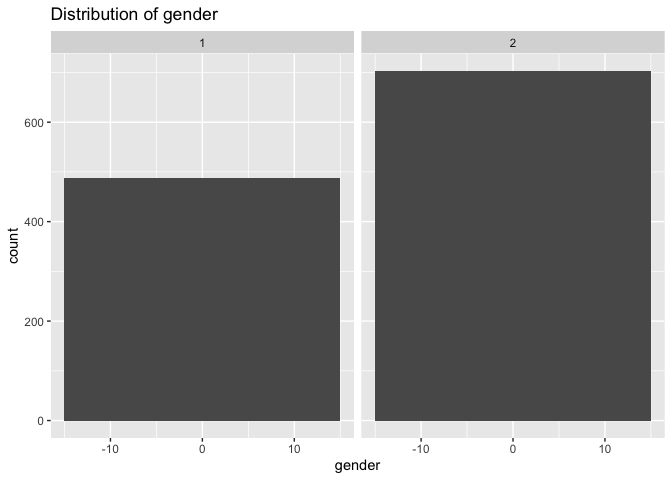
\includegraphics{new_data_files/figure-latex/unnamed-chunk-11-1.pdf}

\hypertarget{conditional-logistic-regression}{%
\subsection{Conditional logistic
regression}\label{conditional-logistic-regression}}

Possible covariates: age (age at the hospital admission time point),
gender (sex\_c coded as 1 for female, 2 for male, 3 is unknown), central
line placement duration (duration)\ldots{}

First, using \texttt{mylogit} to do a logistic regression on the outcome
variable (having blood culture positive) and on the predictor variable
(TPN status). We also want to look at potential confounder so we
included duration as a covariate.

\begin{Shaded}
\begin{Highlighting}[]
\NormalTok{fit.clr }\OtherTok{\textless{}{-}} \FunctionTok{clogit}\NormalTok{(new\_bcp\_status }\SpecialCharTok{\textasciitilde{}}\NormalTok{ new\_tpn\_status }\SpecialCharTok{+}\NormalTok{ age }\SpecialCharTok{+}\NormalTok{ sex\_c }\SpecialCharTok{+} \FunctionTok{strata}\NormalTok{(new\_matching\_period), }\AttributeTok{data =}\NormalTok{ join\_tpn)}

\FunctionTok{round}\NormalTok{(}\FunctionTok{summary}\NormalTok{(fit.clr)}\SpecialCharTok{$}\NormalTok{coef, }\DecValTok{4}\NormalTok{)}
\end{Highlighting}
\end{Shaded}

\begin{verbatim}
##                   coef exp(coef) se(coef)       z Pr(>|z|)
## new_tpn_status  0.7717    2.1633   0.4861  1.5873   0.1124
## age            -0.0103    0.9898   0.0043 -2.4043   0.0162
## sex_cMale       0.0101    1.0101   0.1804  0.0557   0.9556
\end{verbatim}

\begin{Shaded}
\begin{Highlighting}[]
\NormalTok{OR.CI }\OtherTok{\textless{}{-}} \FunctionTok{cbind}\NormalTok{(}\StringTok{"OR"} \OtherTok{=} \FunctionTok{exp}\NormalTok{(}\FunctionTok{coef}\NormalTok{(fit.clr)),}
               \FunctionTok{exp}\NormalTok{(}\FunctionTok{confint}\NormalTok{(fit.clr)))}
\FunctionTok{round}\NormalTok{(OR.CI, }\DecValTok{3}\NormalTok{)}
\end{Highlighting}
\end{Shaded}

\begin{verbatim}
##                   OR 2.5 % 97.5 %
## new_tpn_status 2.163 0.834  5.610
## age            0.990 0.982  0.998
## sex_cMale      1.010 0.709  1.438
\end{verbatim}

Test result discussion:

\begin{enumerate}
\def\labelenumi{\arabic{enumi}.}
\tightlist
\item
  For the exposure predictor \texttt{new\_tpn\_status}, the p-value
  0.1124 is greater than 0.05 which indicates that it is not
  statistically significant. Our model suggests that having total
  parental nutrition does not significantly impact the result of blood
  culture positive. The Odds Ratio of having blood culture positive in
  having TPN compared to non-TPN is eβ = e\^{}0.7717 = 2.163, with a
  95\% CI (0.834, 5.610).
\end{enumerate}

This indicates that: the odds of having blood culture positive in the
total parental nutrition group is 2.163 times the odds of having blood
culture positive in the non-total parental nutrition group

\begin{enumerate}
\def\labelenumi{\arabic{enumi}.}
\setcounter{enumi}{1}
\tightlist
\item
  For the predictor \texttt{age}, the p-value 0.0162 is less than 0.05
  which indicates that it is statistically significant. Our model
  suggests that the age of the patient significantly impacts the result
  of blood culture positive. The exponentiated coefficient for the age
  variable in patients of getting BCP is eβ = e\^{}-0.0103 = 0.990, with
  a 95\% CI (0.982, 0.998).
\end{enumerate}

This indicates that: For every one-year increase in age, the odds of
central-lined patients getting blood culture positive decrease by 1.0\%,
adjusting for TPN, duration, and gender.

\begin{enumerate}
\def\labelenumi{\arabic{enumi}.}
\setcounter{enumi}{2}
\tightlist
\item
  For the predictor \texttt{sex\_c}, the p-value 0.9556 is greater than
  0.05 which indicates that it is not statistically significant. Our
  model suggests that gender does significantly impact the result of
  blood culture positive. The Odds Ratio of being a female and getting
  BCP compares to being a male and getting BCP is eβ = e\^{}0.0101 =
  1.010, with a 95\% CI (0.709, 1.438).
\end{enumerate}

Gender is not a significant covariate in the relationship of getting
blood culture positive.

git config --global http.version HTTP/1.1

\begin{center}\rule{0.5\linewidth}{0.5pt}\end{center}

Notes: model diagnostics, forward selection model Discussion, final
evaluation

May look at the interaction term for age and gender? normality
assumption report the r square : how much the variability take out
duration variable

something else to do: a table a column for cases and for control gender,
age, mean age, p value, tpn cases vs controls package gtsummary to look
at simple p-values

chi-square and t test for each one p-values for each one no need to do
interaction

put in a univariate analysis

discussion section: very small summary of main results, another pgraph
for why you choose the design and the burden, pgraph how you interpret
the findings, did not need to be significant, but why (not enough tpn
people), suprised by why age and gender not associated with the
outcome..

limitation: are we sure we capture every measure correctly

talk about future studies what can be done

english idiom

\end{document}
